% Schematic reconstruction of the visible Q19 diagram (2006 Fujian arts paper).
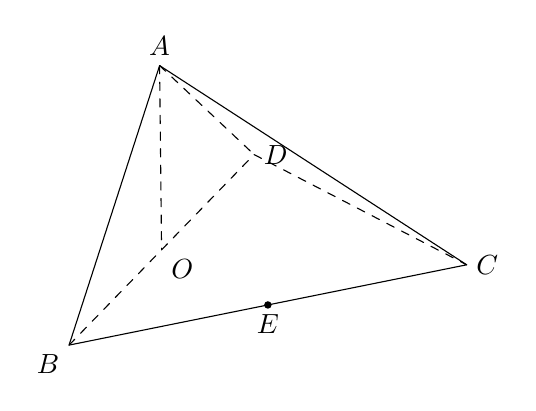
\begin{tikzpicture}[line cap=round,line join=round]
  % Schematic positions only; no lengths or angles are encoded.
  \coordinate (A) at (1.15,3.55);
  \coordinate (B) at (0,0);
  \coordinate (C) at (5.05,1.02);
  \coordinate (D) at (2.35,2.42);
  \coordinate (O) at (1.175,1.21);
  \coordinate (E) at (2.525,0.51);

  % Visible edges
  \draw (A) -- (B) -- (C) -- cycle;

  % Hidden edges and the indicated segment AO
  \draw[dashed] (A) -- (D);
  \draw[dashed] (B) -- (D);
  \draw[dashed] (D) -- (C);
  \draw[dashed] (A) -- (O);

  \fill (E) circle (1.35pt);
  \node[above]       at (A) {$A$};
  \node[below left]  at (B) {$B$};
  \node[right]       at (C) {$C$};
  \node[right]       at (D) {$D$};
  \node[below right] at (O) {$O$};
  \node[below]       at (E) {$E$};
\end{tikzpicture}
